\subsection{Risultati sperimentali}
\label{sec:results}
Proponiamo alcuni risultati sperimentali ottenuti dal package Python contenente gli algoritmi per il calcolo della massima bisimulazione che abbiamo presentato nelle sezioni precedenti. Innanzitutto illustreremo brevemente l'ambiente e gli strumenti con cui sono state prese le misurazioni. Dopodichè presenteremo i risultati in forma di grafici, e tenteremo di evidenziare le differenze tra i vari algoritmi.

\subsubsection{Hardware e strumenti per le misura}
I risultati sono stati misurati su un computer con sistema operativo \emph{CentOS Linux}, architettura x86\_64, processore \emph{Intel(R) Core(TM) i7-4790 CPU} (4 cores, 3.60GHz), e memoria RAM da 16 GB. Per ottenere le misurazioni è stato utilizzato il package Python \emph{timeit}, che presenta alcune caratteristiche che lo rendono un valido strumento per la misurazione del tempo di esecuzione \cite{pythondocs}:
\begin{itemize}
    \item Utilizza la più precisa funzione disponibile sulla piattaforma per la misurazione del tempo trascorso;
    \item Disabilita il \emph{garbage collector}, che potrebbe intervenire in un momento casuale della misurazione introducendo rumore nei risultati;
    \item Esegue lo script preso in esame molte volte in modo da ridurre l'imprecisione dovuta a temporanei sovraccarichi della CPU o della RAM.
\end{itemize}

I dataset su cui abbiamo effettuato le misurazioni sono stati generati utilizzando alcune funzioni del package Python \emph{NetworkX} \cite{networkx}.

\subsubsection{Performance}
Consideriamo alcune tipologie differenti di grafi, e valutiamo il tempo necessario per l'esecuzione degli algoritmi che abbiamo implementato. Nei grafici utilizziamo lungo l'asse delle ascisse una scala data dal valore $|E| \log |V|$, che ci consente di visualizzare in modo più omogeneo i risultati lungo l'asse delle ordinate. Entrambi gli assi variano secondo una scala logaritmica.

\paragraph{Paige-Tarjan, Dovier-Piazza-Policriti} Cominciamo confrontando gli algoritmi di Paige-Tarjan e Dovier-Piazza-Policriti: ci aspettiamo che quest'ultimo risulti asintoticamente più conveniente. Per grafi piccoli invece dovrebbe risultare vincitore l'algoritmo di Paige-Tarjan visto che non richiede l'elaborazione preliminare del rango.

Cominciamo l'esposizione dei risultati con la categoria degli ``alberi bilanciati'', ovvero grafi che possono essere rappresentati nella forma esposta nella Figura \ref{fig:balanced_tree}. Essi sono caratterizzati da due parametri:
\begin{itemize}
    \item \emph{depth}: il numero di livelli (senza contare la \emph{root});
    \item \emph{branching factor}: il numero di successori di ogni nodo (ad eccezione dei nodi nell'ultimo livello).
\end{itemize}

\noindent Generiamo grafi di questo tipo tramite la funzione \verb|balanced_tree| di \emph{NetworkX}, che appunto prende in input questi due parametri.

\begin{figure}
    \centering
    \begin{subfigure}[b]{0.4\textwidth}
        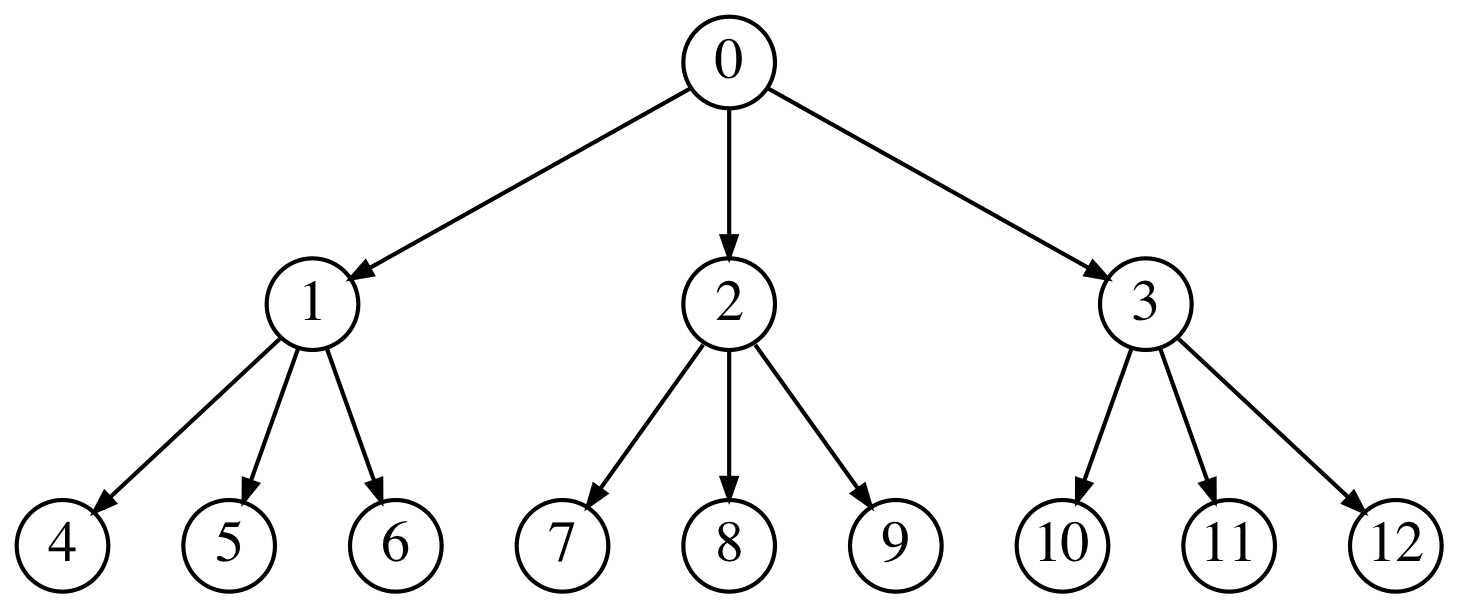
\includegraphics[width=\textwidth]{./sezione3/experimental_results/plots/tree_graph.png}
        \caption{Un albero bilanciato, \emph{depth}=2, \emph{branching factor}=3.}
        \label{fig:balanced_tree}
    \end{subfigure}
    \qquad
    \begin{subfigure}[b]{0.1\textwidth}
        \centering
        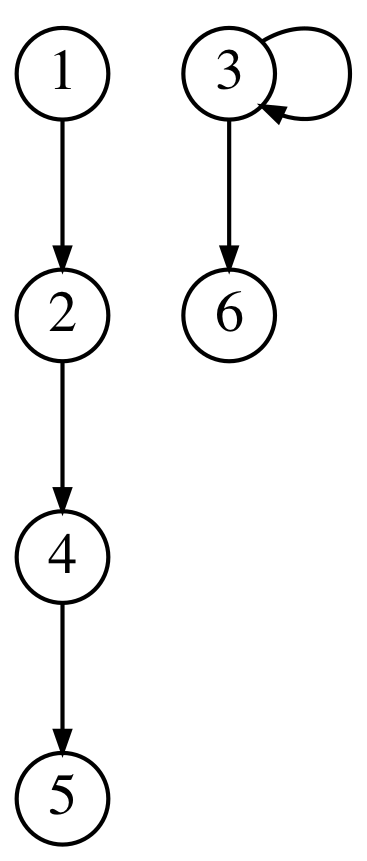
\includegraphics[width=\textwidth]{./sezione3/experimental_results/plots/hopcroft_graph_1.png}
        \caption{Hopcroft, $n=2$}
        \label{fig:hopcroft_graph_1}
    \end{subfigure}
    \qquad \qquad
    \begin{subfigure}[b]{0.2\textwidth}
        \centering
        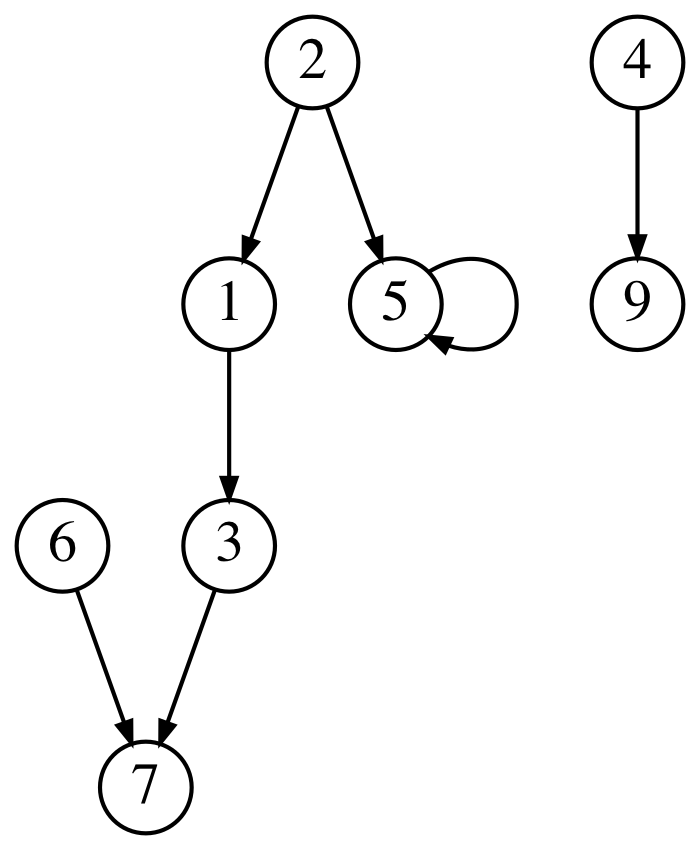
\includegraphics[width=\textwidth]{./sezione3/experimental_results/plots/hopcroft_graph_2.png}
        \caption{Hopcroft, $n=3$}
        \label{fig:hopcroft_graph_2}
    \end{subfigure}
    \caption{Tipologie di grafi su cui abbiamo testato gli algoritmi di Dovier-Piazza-Policriti e Paige-Tarjan.}
\end{figure}

\begin{figure}[b!]
    \centering
    \begin{subfigure}[t]{0.49\textwidth}
        \begin{tikzpicture}
            \begin{axis}[
                axis on top,
                width=\textwidth,
                ytick style={draw=none},
                xtick style={draw=none},
                legend columns=-1,
                legend style={/tikz/every even column/.append style={column sep=0.5cm}},
                legend entries={Paige-Tarjan, Dovier-Piazza-Policriti},
                legend to name=named2,
                xmode=log,
                ymode=log,
                grid=major,
                title={Alberi bilanciati}
            ]
            \addplot table[x=x,y=y] {experiments/time/tree/pta.txt};
            \label{fig:pta_line_tree}
            \addplot table[x=x,y=y] {experiments/time/tree/fba.txt};
            \label{fig:fba_line_tree}
            \end{axis}
        \end{tikzpicture}
    \end{subfigure}
    \hfill
    \begin{subfigure}[t]{0.49\textwidth}
        \begin{tikzpicture}
            \begin{axis}[
                axis on top,
                width=\textwidth,
                ytick style={draw=none},
                xtick style={draw=none},
                grid=major,
                xmode=log,
                ymode=log,
                title={Grafi di Hopcroft}
            ]
            \addplot table[x=x,y=y] {experiments/time/hopcroft/pta.txt};
            \addplot table[x=x,y=y] {experiments/time/hopcroft/fba.txt};
            \end{axis}
        \end{tikzpicture}
    \end{subfigure}
    \ref*{named2}
    \caption{Tempo di esecuzione degli algoritmi di Dovier-Piazza-Policriti e Paige-Tarjan su alberi bilanciati (destra) e automi proposti da Hopcroft (sinistra). Lungo l'asse delle ascisse (logaritmico) varia la quantità $|E|\log|V|$, mentre sull'asse delle ordinate (logaritmico) è riportato il tempo di esecuzione dell'algoritmo in secondi.}
    \label{fig:pta_vs_fba}
\end{figure}

Dal grafico rappresentato nella parte sinistra della Figura \ref{fig:pta_vs_fba} possiamo osservare che l'algoritmo di Dovier-Piazza-Policriti risulta asintoticamente più efficiente, a partire da un certo valore di $|E| \log |V|$. Sebbene infatti la metodologia sia più ``rifinita'' dell'approccio di Paige-Tarjan, lo sforzo iniziale per il calcolo del rango è apprezzabile, soprattutto se consideriamo il linguaggio in cui l'algoritmo è stato implementato. Abbiamo però la conferma che per valori alti di $|E| \log |V|$, per questa tipologia di grafo, si ottengono i risultati previsti.

La seconda tiplogia di grafi che consideriamo è tratta dall'articolo in cui viene presentato l'algoritmo di Dovier-Piazza-Policriti, ed è un esempio di automa proposto originariamente da Hopcroft \cite{hopcroft}. Nelle Figure \ref{fig:hopcroft_graph_1} e \ref{fig:hopcroft_graph_2} ne visualizziamo alcune realizzazioni. Nella parte destra della Figura \ref{fig:pta_vs_fba} sono riportati i risultati ottenuti dagli algoritmi. Osserviamo nuovamente che l'algoritmo di Dovier-Piazza-Policriti risulta asintoticamente più conveniente.

\paragraph{Algoritmo incrementale} Proseguiamo l'esposizione dei risultati sperimentali ottenuti utilizzando il pacchetto \texttt{BisPy} con un confronto tra gli algoritmi di Paige-Tarjan e Dovier-Piazza-Policriti (cui ci riferiremo in questa sezione con ``algoritmi \emph{from scratch}'', in quanto ricalcolano da zero la massima bisimulazione) e l'algoritmo incrementale di Saha. L'obiettivo di questo confronto è verificare di quanto e in quali casi l'algoritmo incrementale risulti più efficiente nel ricalcolare la massima bisimulazione in seguito all'aggiunta di un nuovo arco, rispetto ad un algoritmo che non sfrutti le informazioni relative alla massima bisimulazione prima della modifica. Rammentiamo la complessità dell'algoritmo di Saha, ottenuta nella Sezione \ref{sec:saha_complexity} come la somma delle varie fasi di cui si compone il procedimento:
\begin{align}\label{eq:saha}
    T_{\text{Saha}} = O(|E_1|\log|V_1|) &+ O(|\Delta_{\wf}\log|\Delta_{\wf}|) + O(|E_{\nwf}| + |V_{\nwf}|)\\
    &+ O(|E_2||V_2|) + O(|E_2|\log|V_2|)
\end{align}

$\Delta_\nwf$ è l'insieme di nodi \emph{non-well-founded} il cui rango è cambiato in seguito all'inserimento del nuovo arco; $E_1,V_1$ e $E_2,V_2$ sono rispettivamente nodi e archi appartenenti al sottografo di $G$ composto dai nodi modificati durante le fasi 1. (\funcname{split}) e 2. (\funcname{merge}); $E_{\nwf}$, $V_{\nwf}$ sono rispettivamente archi e nodi del sottografo \emph{non-well-founded} di $G$. Si osservi che numerosi termini possono diventare molto facilmente ``problematici'', e rendere quindi l'algoritmo incrementale meno efficiente del ricalcolo da zero della massima bisimulazione. In questa breve analisi presenteremo i risultati su alcune tipologie di grafo, e ne verificheremo la coerenza con l'analisi proposta nelle sezioni precedenti.

\begin{figure}[t!]
    \centering
    \begin{subfigure}[t]{0.48\textwidth}
        \begin{tikzpicture}
            \begin{axis}[
                axis on top,
                width=\textwidth,
                legend columns=-1,
                legend style={/tikz/every even column/.append style={column sep=0.5cm}},
                legend entries={Paige-Tarjan, Dovier-Piazza-Policriti, Saha},
                legend to name=named,
                ytick style={draw=none},
                xtick style={draw=none},
                xlabel={\texttt{n}},
                xlabel style={font=\large},
                ylabel={Secondi},
                ylabel style={font=\large},
                xmode=log,
                ymode=log,
                grid=major,
                title={\texttt{p}$=0.0001$}
            ]
            \addplot table[x=x,y=y] {experiments/time/saha/random/mean_0_0.txt};
            \addplot table[x=x,y=y] {experiments/time/saha/random/mean_0_1.txt};
            \addplot table[x=x,y=y] {experiments/time/saha/random/mean_0_2.txt};
        \end{axis}
        \end{tikzpicture}
    \end{subfigure}
    \hfill
    \begin{subfigure}[t]{0.48\textwidth}
        \begin{tikzpicture}
            \begin{axis}[
                axis on top,
                width=\textwidth,
                ytick style={draw=none},
                xtick style={draw=none},
                xlabel={\texttt{n}},
                xlabel style={font=\large},
                ylabel={Secondi},
                ylabel style={font=\large},
                xmode=log,
                ymode=log,
                grid=major,
                title={\texttt{p}$=0.0005$}
            ]
            \addplot table[x=x,y=y] {experiments/time/saha/random/mean_1_0.txt};
            \addplot table[x=x,y=y] {experiments/time/saha/random/mean_1_1.txt};
            \addplot table[x=x,y=y] {experiments/time/saha/random/mean_1_2.txt};
        \end{axis}
        \end{tikzpicture}
    \end{subfigure}
    \ref*{named}
    \caption{Tempo medio in secondi (su un campione di 100 grafi) impiegato per l'aggiornamento della massima bisimulazione in seguito all'aggiunta di un arco generato in modo randomico. Lungo l'asse delle ascisse varia il numero di nodi del grafo binomiale.}
    \label{fig:saha_results_random}
\end{figure}

Per il primo esperimento consideriamo grafi randomici di Erdős-Rényi (o \emph{grafi binomiali}), ovvero grafi contenenti un numero arbitrario \verb|n| di nodi, per cui presa una coppia qualsiasi $u,v \in V$ si ha $\langle u,v\rangle \in E$ con probabilità \verb|p| $\leq 1$. Sono stati generati 100 grafi tramite la funzione \verb|fast_gnp_random_graph| di \emph{NetworkX}, che prende in ingresso i parametri \texttt{n,p}, e per ognuno è stato aggiunto un arco scelto randomicamente tra quelli non esistenti. Infine si è verificato il tempo di esecuzione per gli algoritmi di Paige-Tarjan, Dovier-Piazza-Policriti e Saha (Figura \ref{fig:saha_results_random}). L'algoritmo incrementale risulta mediamente più conveniente per entrambi i valori di \texttt{p} considerati, ma è evidente che con l'aumento di questo parametri la convenienza si riduce in modo significativo. Tale comportamento è coerente con \eqref{eq:saha}. Nella Figura \ref{fig:saha_scatter_random} sono riportati i 100 risultati per due coppie (\texttt{n,p}). Questa visualizzazzione ci consente di osservare che non sempre l'algoritmo incrementale è il più conveniente: per i valori considerati viene saltuariamente superato dall'algoritmo di Paige-Tarjan.

\begin{figure}[H]
    \centering
    \begin{subfigure}[t]{\textwidth}
        \begin{tikzpicture}
            \begin{axis}[
                axis on top,
                width=\textwidth,
                height=6cm,
                legend columns=-1,
                legend style={/tikz/every even column/.append style={column sep=0.5cm}},
                legend entries={Paige-Tarjan, Dovier-Piazza-Policriti, Saha},
                legend to name=named5,
                ytick style={draw=none},
                xtick style={draw=none},
                xtick={0.0,20.0,40.0,60.0,80.0,100.0},
                xticklabels={0,20,40,60,80,100},
                xlabel={\texttt{n}},
                xlabel style={font=\large},
                ylabel={Secondi},
                ylabel style={font=\large},
                grid=major,
                title={\texttt{n}=2000, \texttt{p}=0.0001},
                only marks
            ]
            \addplot+[mark=o,ultra thin,mark options={scale=1}] table[x=x,y=y] {experiments/time/saha/random/scatter_0_0.txt};
            \addplot+[mark=asterisk,ultra thin,mark options={scale=1}] table[x=x,y=y] {experiments/time/saha/random/scatter_0_1.txt};
            \addplot+[mark=square,ultra thin,mark options={scale=1}] table[x=x,y=y] {experiments/time/saha/random/scatter_0_2.txt};
            \addplot+[
                domain=0:100,
                samples=100,
                no marks,
                sharp plot,
                color=blue,
                line width=1pt,
                solid
            ]
            {0.02367323};
            \addplot+[
                domain=0:100,
                samples=100,
                no marks,
                sharp plot,
                color=red,
                line width=1pt,
                solid
            ]
            {0.05305607};
            \addplot+[
                domain=0:100,
                samples=100,
                no marks,
                sharp plot,
                color=brown,
                line width=1pt,
                solid
            ]
            {0.01112568};
        \end{axis}
        \end{tikzpicture}
    \end{subfigure}
    \begin{subfigure}[t]{\textwidth}
        \begin{tikzpicture}
            \begin{axis}[
                axis on top,
                width=\textwidth,
                height=6cm,
                ytick style={draw=none},
                xtick style={draw=none},
                xtick={0.0,20.0,40.0,60.0,80.0,100.0},
                xticklabels={0,20,40,60,80,100},
                xlabel={\texttt{n}},
                xlabel style={font=\large},
                ylabel={Secondi},
                ylabel style={font=\large},
                grid=major,
                title={\texttt{n}=2000, \texttt{p}=0.0005},
                only marks
            ]
            \addplot+[mark=o,ultra thin,mark options={scale=1}] table[x=x,y=y] {experiments/time/saha/random/scatter_1_0.txt};
            \addplot+[mark=asterisk,ultra thin,mark options={scale=1}] table[x=x,y=y] {experiments/time/saha/random/scatter_1_1.txt};
            \addplot+[mark=square,ultra thin,mark options={scale=1}] table[x=x,y=y] {experiments/time/saha/random/scatter_1_2.txt};
            \addplot+[
                domain=0:100,
                samples=100,
                no marks,
                sharp plot,
                color=blue,
                line width=1pt,
                solid
            ]
            {0.06129174};
            \addplot+[
                domain=0:100,
                samples=100,
                no marks,
                sharp plot,
                color=red,
                line width=1pt,
                solid
            ]
            {0.07297469};
            \addplot+[
                domain=0:100,
                samples=100,
                no marks,
                sharp plot,
                color=brown,
                line width=1pt,
                solid
            ]
            {0.03012856};
        \end{axis}
        \end{tikzpicture}
    \end{subfigure}
    \ref*{named5}
    \caption{Tempo di esecuzione per i tre algoritmi considerati per i 100 grafi generati in modo randomico menzionati nel primo esperimento, per due coppie (\texttt{n,p}) = (2000,0.0001) (sopra), (2000,0.0005) (sotto). Le linee continue rappresentano la media registrata da ognuno dei tre algoritmi.}
    \label{fig:saha_scatter_random}
\end{figure}

Per il secondo esperimento abbiamo ritenuto interessante esaminare i risultati ottenuti su grafi con una certa struttura. Per quest motivo sono stati considerati degli \emph{alberi bilanciati}, una tipologia di grafi che abbiamo già descritto sommariamente nel paragrafo precedente. Abbiamo generato 100 archi in modo randomico (escludendo quelli già presenti) ed abbiamo utilizzato i tre algoritmi presentati in questo lavoro per aggiornare la massima bisimulazione, al fine di confrontare il tempo di esecuzione degli algoritmi \emph{from scratch} e l'algoritmo incrementale. I risultati sono rappresentati nella parte sinistra della Figura \ref{fig:saha_results_tree}. Ad una prima analisi del grafico sembra che non vi sia una particolare convenienza nell'utilizzo dell'algoritmo di Saha; questa impressione è però in parte sbagliata, è necessario ricordate che gli archi sono generati in modo randomico e che il tempo di esecuzione è estremamente suscettibile alla tipologia di arco in cui consiste la modifica. La situazione è rappresentata meglio nella parte destra della Figura \ref{fig:saha_results_tree}, in cui abbiamo diviso gli archi in categorie in base alla seguente funzione:
\begin{gather*}
    \Delta v(\langle x,y \rangle) = \texttt{Depth}(x) - \texttt{Depth}(y)
\end{gather*}
dove \texttt{Depth}$(x)$ è il livello dell'albero in cui si trova il nodo $x$. Per chiarezza abbiamo rappresentato solamente l'andamento temporale dell'algoritmo di Paige-Tarjan, e dell'algoritmo di Saha per gli archi con $\Delta v \in \{-1,0,3\}$. Si oosservi che per $\Delta v = -1$ il tempo di esecuzione è molto basso in quanto non viene introdotto alcun cambiamento. Per $\Delta v = 0$ invece il tempo medio di esecuzione è addirittura peggiore di quello registrato dall'algoritmo di Paige-Tarjan, in quanto la bisimulazione massima viene cambiata in modo molto significativo. Questo esperimento mostra come una valutazione probabilistica della tipologia di arco in cui consiste la modifica del grafo sia fondamentale per decidere quale algoritmo utilizzare nelle applicazioni pratiche.

\begin{figure}[H]
    \centering
    \begin{subfigure}[t]{0.48\textwidth}
        \begin{tikzpicture}
            \begin{axis}[
                axis on top,
                width=\textwidth,
                ytick style={draw=none},
                xtick style={draw=none},
                legend style={fill=white,opacity=0.8, at={(0,0.58)},anchor=south west, legend columns=1},
                xlabel={\texttt{n}},
                xlabel style={font=\large},
                ylabel={Secondi},
                ylabel style={font=\large},
                xtick={5.0,6.0,7.0,8.0,9.0,10.0},
                xticklabels={5,6,7,8,9,10},
                ymode=log,
                grid=major,
                title={Tempo medio su \emph{balanced tree}}
            ]
            \addplot table[x=x,y=y] {experiments/time/saha/tree/first/mean_0_0.txt};
            \addlegendentry{Paige-Tarjan}
            \addplot table[x=x,y=y] {experiments/time/saha/tree/first/mean_0_1.txt};
            \addlegendentry{DPP}
            \addplot table[x=x,y=y] {experiments/time/saha/tree/first/mean_0_2.txt};
            \addlegendentry{Saha}
        \end{axis}
        \end{tikzpicture}
    \end{subfigure}
    \hfill
    \begin{subfigure}[t]{0.48\textwidth}
        \begin{tikzpicture}
            \begin{axis}[
                axis on top,
                width=\textwidth,
                legend style={fill=white,opacity=0.8, at={(0,0.45)},anchor=south west, legend columns=1},
                xlabel={\texttt{n}},
                xlabel style={font=\large},
                ylabel={Secondi},
                ylabel style={font=\large},
                yminorticks=false,
                xtick={5.0,6.0,7.0,8.0,9.0,10.0},
                xticklabels={5,6,7,8,9,10},
                ymode=log,
                grid=major,
                title={Raggruppamento per tipo di arco}
            ]
            \addplot table[x=x,y=y] {experiments/time/saha/tree/first/mean_0_0.txt};
            \addlegendentry{Paige-Tarjan}
            %\addplot table[x=x,y=y] {experiments/time/saha/tree/first/mean_0_1.txt};
            %\addplot table[x=x,y=y] {experiments/time/saha/tree/second/data1.txt};
            %\addplot table[x=x,y=y] {experiments/time/saha/tree/second/data2.txt};
            \addplot table[x=x,y=y] {experiments/time/saha/tree/second/data3.txt};
            \addlegendentry{Saha $\Delta v = \hphantom{-}3$}
            \addplot table[x=x,y=y] {experiments/time/saha/tree/second/datam0.txt};
            \addlegendentry{Saha $\Delta v = \hphantom{-}0$}
            \addplot table[x=x,y=y] {experiments/time/saha/tree/second/datam1.txt};
            \addlegendentry{Saha $\Delta v = -1$}
            %\addplot table[x=x,y=y] {experiments/time/saha/tree/second/datam2.txt};
            %\addplot table[x=x,y=y] {experiments/time/saha/tree/second/datam3.txt};
            %\addplot table[x=x,y=y] {experiments/time/saha/tree/second/datam4.txt};
            %\addlegendentry{Saha $\Delta v = -4$}
        \end{axis}
        \end{tikzpicture}
    \end{subfigure}
    \caption{Tempo medio in secondi (su un campione di 100 archi) impiegato per l'aggiornamento della massima bisimulazione in seguito all'aggiunta di un arco generato in modo randomico, su \emph{balanced tree} con \emph{depth} variabile e \emph{branching factor} fissato a 2. Nell'immagine a sinistra (l'algoritmo di Dovier-Piazza-Policriti è stato abbreviato in ``DPP'') abbiamo rappresentato i risultati complessivi, nell'immagine a destra abbiamo diviso gli archi in categorie a seconda della distanza (in livelli) tra i due nodi corrispondenti, ed abbiamo poi preso il tempo medio di questi ``cluster''.}
    \label{fig:saha_results_tree}
\end{figure}

\subsubsection{Dimensione della massima bisimulazione}
Terminiamo la sezione relativa ai risultati sperimentali con un'ultima analisi che potrebbe essere di qualche interesse nella prospettiva di ciò che abbiamo presentato nella Sezione \ref{sec:applications}. Verificheremo l'andamento del numero di classi di equivalenza nella massima bisimulazione per i grafi randomici di Erdős-Rényi considerati poco sopra. Considereremo valori piccoli di \verb|p|, in quanto avvicinandoci ad 1 otteniamo grafi sempre più ``completi'' di interesse molto basso nella pratica. Nella Figura \ref{fig:bisi_size} abbiamo considerato tre diversi valori per il parametro \verb|n|, e quattro valori per il parametro \verb|p|.

\begin{figure}[t!]
    \begin{center}
        \begin{subfigure}[b]{0.3\textwidth}
            \begin{tikzpicture}[scale=1.3]
                \begin{axis}[
                    axis on top,
                    width=\textwidth,
                    legend columns=-1,
                    legend style={/tikz/every even column/.append style={column sep=0.5cm}},
                    legend entries={$p=0.01$, $p=0.05$, $p=0.1$, $p=0.2$},
                    legend to name=named,
                    tick pos=both,
                    xtick style={color=black},
                    ytick style={color=black},
                    grid=both,
                    title={$n=10$}
                ]
                \addplot[scatter, scatter/classes={
                    a={mark=asterisk,blue},
                    b={mark=diamond,red},
                    c={mark=square,green},
                    d={mark=triangle,yellow}
                    }, only marks, scatter src=explicit symbolic] table[y=y,meta=label] {experiments/dimension/dim/result10.txt};
                \end{axis}
            \end{tikzpicture}
        \end{subfigure}
        \begin{subfigure}[b]{0.3\textwidth}
            \begin{tikzpicture}[scale=1.3]
                \begin{axis}[
                    axis on top,
                    width=\textwidth,
                    tick pos=both,
                    xtick style={color=black},
                    ytick style={color=black},
                    grid=both,
                    title={$n=100$}
                ]
                \addplot[scatter, scatter/classes={
                    a={mark=asterisk,blue},
                    b={mark=diamond,red},
                    c={mark=square,green},
                    d={mark=triangle,yellow}
                    }, only marks, scatter src=explicit symbolic] table[y=y,meta=label] {experiments/dimension/dim/result100.txt};
                \end{axis}
            \end{tikzpicture}
        \end{subfigure}
        \begin{subfigure}[b]{0.3\textwidth}
            \begin{tikzpicture}[scale=1.3]
                \begin{axis}[
                    axis on top,
                    width=\textwidth,
                    tick pos=both,
                    xtick style={color=black},
                    ytick style={color=black},
                    grid=both,
                    title={$n=1000$}
                ]
                \addplot[scatter, scatter/classes={
                    a={mark=asterisk,blue},
                    b={mark=diamond,red},
                    c={mark=square,green},
                    d={mark=triangle,purple}
                    }, only marks, scatter src=explicit symbolic] table[y=y,meta=label] {experiments/dimension/dim/result1000.txt};
                    \label[a]{fig:bisi_size_1000_p001}
                    \label[b]{fig:bisi_size_1000_p005}
                    \label[c]{fig:bisi_size_1000_p01}
                    \label[d]{fig:bisi_size_1000_p02}
                \end{axis}
            \end{tikzpicture}
        \end{subfigure}
        \ref*{named}
    \end{center}
    \caption{Numero di classi di equivalenza della massima bisimulazione per grafi generati in modo casuale, normalizzato rispetto al numero di nodi nel grafo. Ad ogni \emph{tick} sull'asse delle ascisse corrisponde un grafo generato in modo casuale. Lungo l'asse delle ordinate è riportato il numero di blocchi della bisimulazione massima.}
    \label{fig:bisi_size}
\end{figure}

Per ogni combinazione di \verb|n|,\verb|p| abbiamo generato 100 grafi binomiali con la funzione \verb|fast_gnp_random_graph| del pacchetto \emph{NetworkX}, e ne abbiamo calcolata la massima bisimulazione con l'algoritmo di \emph{Dovier-Piazza-Policriti}. Nei grafici abbiamo visualizzato la quantità $\frac{|V / \equiv|}{|V|}$, ovvero il rapporto tra il numero di classi di equivalenza nella massima bisimulazione ed il numero di nodi del grafo: questa quantità potrebbe essere considerata come il fattore di riduzione che otteniamo quanto sostuitiamo al grafo originale la sua contrazione secondo la massima bisimulazione.

Per \verb|n=10| la quantità che stiamo valutando varia molto tra 1 (10 classi di equivalenza, nessuna riduzione) e 0.1 (tutti i nodi sono bisimili, riduzione massima). Per valori più grandi la variabilità si riduce, e per \verb|n=1000| il fattore si schiaccia decisamente verso 0.001 (un'unica partizione).
